\chapter{User and Group Management}

Gravwell implements users and groups in a manner very similar to Unix.
Each user has a username, a real name, and a numeric UID. Each group has
a name, a numeric group ID, and a list of member UIDs. As in Unix, users
can belong to multiple groups. The biggest difference from Unix is that
a given item (such as a resource) can often be made accessible to
members of \emph{multiple} groups, where Unix only allows one.

Many user actions generate entries in the webserver's logs. Provided
the webserver's Log-Level parameter has been set to \code{INFO}, the
file \code{/opt/gravwell/log/web/info.log} will contain very verbose logs
of user logins, user searches, and more.

\section{Managing Users}
\index{Users}\index{GUI!users}
The Gravwell GUI includes an admin-only page for managing users,
located in the menu under the Administrator section. From this page, an
administrator can create new users, modify existing users, or delete
users. Figure \ref{fig:fresh-users} shows the User page on a freshly-installed
Gravwell system; the only extant user is the default ``admin''.

\begin{figure}
	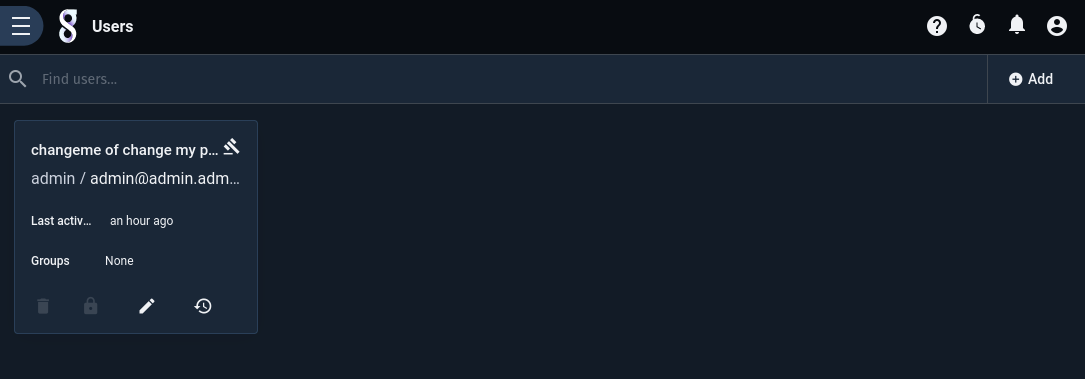
\includegraphics{images/users-admin.png}
	\caption{A Freshly-Installed System's User List}
	\label{fig:fresh-users}
\end{figure}

Clicking the `Add' button in the upper right brings up a dialog to
create a new user, as shown in Figure \ref{fig:newuser}. Note the 
`Administrator' checkbox at the bottom of the dialog. If this
box is checked, the user will receive administrator-level privileges.
Take care when selecting this option!


\begin{figure}
	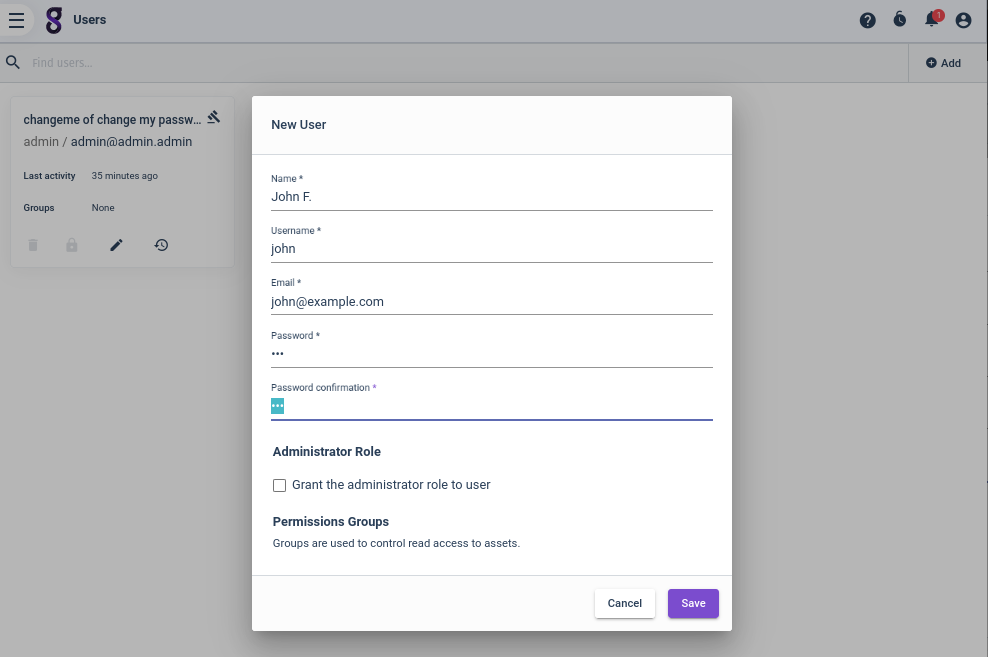
\includegraphics{images/newuser.png}
	\caption{New User Dialog}
	\label{fig:newuser}
\end{figure}


Each user information tile has four icons across the bottom, as shown in Figure \ref{fig:usertile}.
Selecting the trashcan icon will delete the user (prompting for
confirmation). The padlock icon will lock the user account, logging out
any sessions they may currently have and preventing them from logging in
again until the account is unlocked; this is a good way to deal with
misbehaving users. Both of these icons are disabled for the `admin'
user.

\begin{figure}
	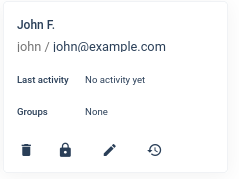
\includegraphics[width=0.5\linewidth]{images/usertile.png}
	\caption{The User Information Tile}
	\label{fig:usertile}
\end{figure}

The pencil icon brings up a dialog to edit the existing user, as shown in Figure \ref{fig:edituser}.
This allows you to reset the user's password, change their personal
information, or even make them an administrator if needed.

\begin{figure}
	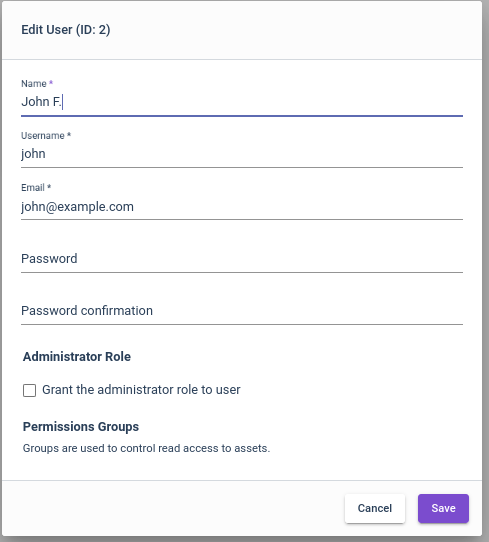
\includegraphics[width=0.55\linewidth]{images/edituser.png}
	\caption{Editing User Information}
	\label{fig:edituser}
\end{figure}

Finally, the clock icon brings up the user's search history, as shown in Figure \ref{fig:userhistory}.
This can be useful when attempting to help a user figure out why their searches
aren't working, or to keep an eye on what users are trying to extract
from your data.

\begin{figure}
	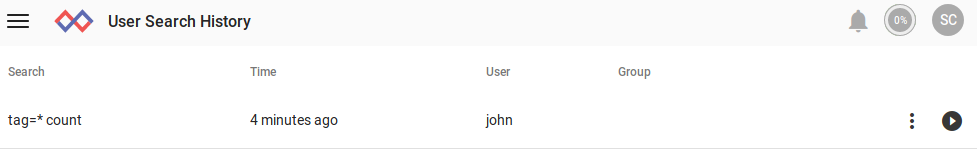
\includegraphics[width=0.9\linewidth]{images/userhistory.png}
	\caption{User Search History}
	\label{fig:userhistory}
\end{figure}

\section{Managing Groups}
\index{Groups}\index{GUI!groups}
Group management is very similar to user management. The Groups page in
the Administration section of the menu will initially show no groups, as in
Figure \ref{fig:fresh-groups}

\begin{figure}[H]
	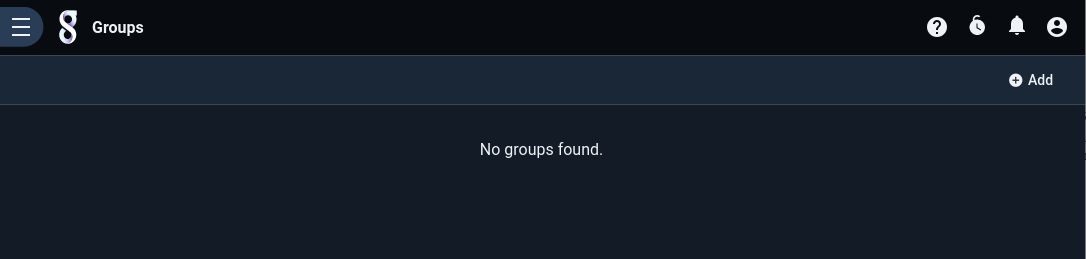
\includegraphics{images/empty-groups.png}
	\caption{A Freshly-Installed System's Group List}
	\label{fig:fresh-groups}
\end{figure}

A group can be added by clicking the `Add' button and filling out the
form, optionally selecting any users which should be members of the new
group, as shown in Figure \ref{fig:newgroup}

\begin{figure}
	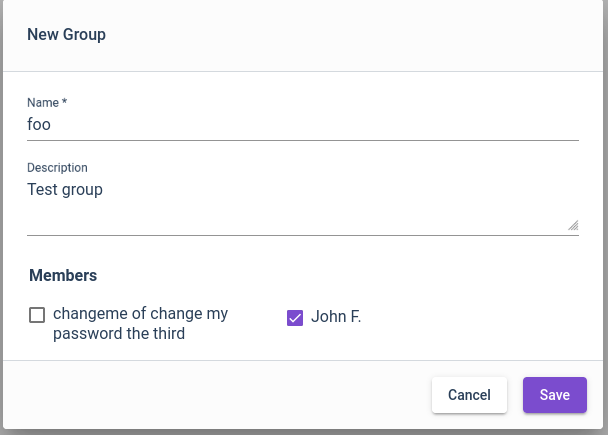
\includegraphics[width=0.6\linewidth]{images/newgroup.png}
	\caption{New Group Dialog}
	\label{fig:newgroup}
\end{figure}

Once created, a group's tile has three action icons as seen in Figure \ref{fig:grouptile}.
The trashcan icon deletes the group. The pencil icon allows the group
to be renamed or for members to be added/deleted. The clock icon shows
the history of searches which have been run which were accessible to
this group.

\begin{figure}
	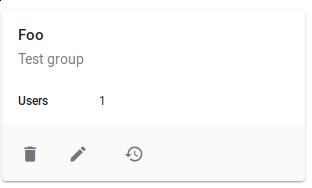
\includegraphics[width=0.5\linewidth]{images/grouptile.png}
	\caption{The Group Information Tile}
	\label{fig:grouptile}
\end{figure}

\clearpage
\section{Hands-on Lab: Managing Users and Groups}

First, launch a Gravwell webserver+indexer container:

\begin{Verbatim}[breaklines=true]
docker run --rm --net gravnet -p 8080:80 -d --name gravwell gravwell:base
\end{Verbatim}

Log into the web GUI (\href{http://localhost:8080}{http://localhost:8080}) and try the following tasks using the GUI:

\begin{enumerate}
\item
  Create a new user for yourself.
\item
  Create a new group and add your user to the group.
\item
  Log in as your user in a separate incognito window. From the admin
  account, lock your user account. What happened?
\end{enumerate}

To clean up after the experiment, run:

\code{docker kill \$(docker ps -a -q)}

\clearpage
\section{Access Control}

Capability Based Access Control (CBAC) is a feature access system that enables users and groups to be configured with fine-grained access to various Gravwell features. For example, using CBAC, a user can be configured to have access to search, but not resources or kits. Additionally, CBAC can be used to define which tags are available to users and groups.

CBAC is based around a deny-all default policy. Capabilities and tag access must be granted to each user (or group a user belongs to) in order to access those features. Admin users are not restricted by CBAC and always have full system access.

\subsection{Enabling CBAC}

CBAC is enabled by adding the following clause to the global section of the webserver's \code{gravwell.conf} and restarting the webserver:

\begin{verbatim}
Enable-CBAC=true
\end{verbatim}

Because CBAC has a deny-all default policy, if this is the first time enabling CBAC, \emph{all} non-admin users will begin with no capabilities or tag access. 

\subsection{Granting Capabilities to Users and Groups}

Admin users can grant capability and tag access to both users and groups via the Users and Groups pages in the Administrator section of the main menu, as shown in Figure \ref{fig:capability-editor}.

\begin{figure}
	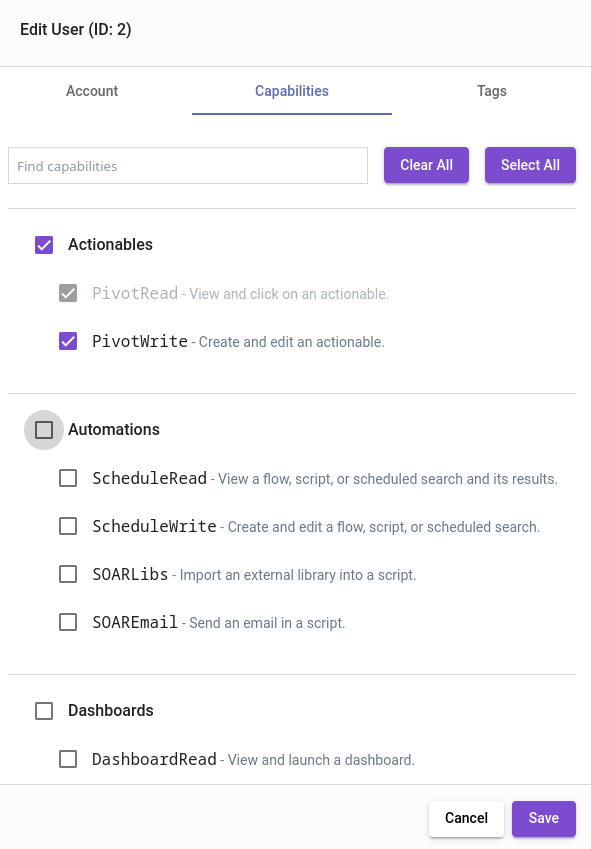
\includegraphics[width=0.5\linewidth]{images/cbac_user.png}
	\caption{Editing a user's access permissions.}
	\label{fig:capability-editor}
\end{figure}

When creating or editing a user or group, select the ``Capabilities'' tab and select the capabilities you wish to add. Users that are part of a group will also inherit capabilities from that group.

Tag access is configured by selecting the Tags tab, and selecting the tags the user or group has access to.

Users that don't have access to a particular feature will see a menu system with those features disabled. For example, a user that does not have access to dashboard or data ingest will see a menu system like Figure \ref{fig:capability-menu}

\begin{figure}
	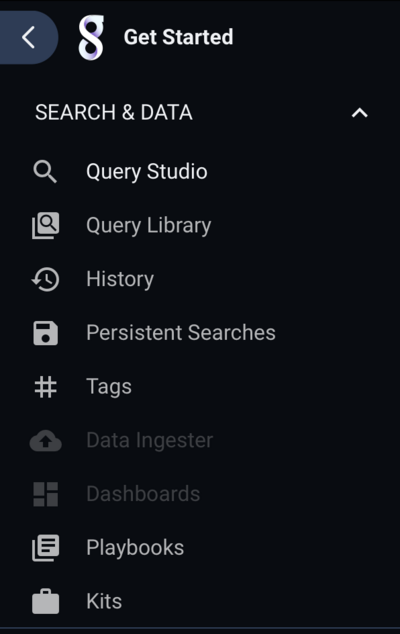
\includegraphics[width=0.5\linewidth]{images/cbac_menu.png}
	\caption{A CBAC-restricted main menu}
	\label{fig:capability-menu}
\end{figure}

\subsection{Granting Capabilities in Practice}

In practice, it is less common to grant capabilities to individual users; instead, administrators create groups with specific roles and assign users to those groups. For example, creating a group named ``IT Users'' that has access to IT-related tags (syslog, router logs, firewall logs, etc.), and a group named ``Incident Response Users'' that has access to IDS and other security related data, allows the admin to grant access to users based on their role. Users that need access to both IT and Incident response data in this example can simply be added to both groups.  In essence CBAC grants applied to groups implements RBAC (role based access control).

\subsection{Determining a CBAC Grant}

A user is granted access based on the combination of capabilities and tags that are granted directly to the user and also those granted to any groups the user belongs to.

For example, user ``Bob'' has access to Search and Resources (but nothing else), and the \code{gravwell} tag. Bob is also a member of a group that grants access to Dashboards and the \code{default} tag. As a result, ``Bob'' has access to Search, Resources, and Dashboards, and both the \code{gravwell} and \code{default} tags.

\subsection{CBAC Restrictions in Search}

CBAC capabilities also apply to search. A user that does not have access to resources will still be able to invoke the \code{lookup} module (and other resource-based modules), but that module will list no resources as being available. Similarly, macros, auto extractors, and related features in the \code{anko} and legacy \code{eval} modules will be restricted based on the user's CBAC grants.

\subsection{Caveats}

Some capabilities require both read and write grants in order to function correctly, such as Resources and Playbooks.

The GUI automatically selects read access for a given feature if any of the write capabilities for that feature are selected. If write-only access is needed, you must use the Gravwell command line tool to configure the capability.

